\documentclass[10pt,fleqn]{article} % Default font size and left-justified equations
\usepackage[%
    pdftitle={Informatique : capteur rayonnement},
    pdfauthor={Xavier Pessoles}]{hyperref}

%%%%%%%%%%%%%%%%%%%%%%%%%%%%%%%%%%%%%%%%%
% Original author:
% Mathias Legrand (legrand.mathias@gmail.com) with modifications by:
% Vel (vel@latextemplates.com)
% License:
% CC BY-NC-SA 3.0 (http://creativecommons.org/licenses/by-nc-sa/3.0/)
%%%%%%%%%%%%%%%%%%%%%%%%%%%%%%%%%%%%%%%%%



%----------------------------------------------------------------------------------------
%	MAIN TABLE OF CONTENTS
%----------------------------------------------------------------------------------------


% Part text styling
\titlecontents{part}[0cm]
{\addvspace{20pt}\centering\large\bfseries}
{}
{}
{}

% Chapter text styling
\titlecontents{chapter}[1.25cm] % Indentation
{\addvspace{12pt}\large\sffamily\bfseries} % Spacing and font options for chapters
{\color{bleuxp!60}\contentslabel[\Large\thecontentslabel]{1.25cm}\color{bleuxp}} % Chapter number
{\color{bleuxp}}  
{\color{bleuxp!60}\normalsize\;\titlerule*[.5pc]{.}\;\thecontentspage} % Page number

% Section text styling
\titlecontents{section}[1.25cm] % Indentation
{\addvspace{3pt}\sffamily\bfseries} % Spacing and font options for sections
{\color{bleuxp!60}\contentslabel[\thecontentslabel]{1.25cm} \color{bleuxp}} % Section number
{\color{bleuxp}}
{\hfill\color{bleuxp!60}\thecontentspage} % Page number
[]

% Subsection text styling
\titlecontents{subsection}[1.25cm] % Indentation
{\addvspace{1pt}\sffamily\small} % Spacing and font options for subsections
{\contentslabel[\thecontentslabel]{1.25cm}} % Subsection number
{}
{\ \titlerule*[.5pc]{.}\;\thecontentspage} % Page number
[]


% Subsection text styling
\titlecontents{subsubsection}[1.25cm] % Indentation
{\addvspace{1pt}\sffamily\small} % Spacing and font options for subsections
{\contentslabel[\thecontentslabel]{1.25cm}} % Subsection number
{}
{\ \titlerule*[.5pc]{.}\;\thecontentspage} % Page number
[]

% List of figures
\titlecontents{figure}[0em]
{\addvspace{-5pt}\sffamily}
{\thecontentslabel\hspace*{1em}}
{}
{\ \titlerule*[.5pc]{.}\;\thecontentspage}
[]

% List of tables
\titlecontents{table}[0em]
{\addvspace{-5pt}\sffamily}
{\thecontentslabel\hspace*{1em}}
{}
{\ \titlerule*[.5pc]{.}\;\thecontentspage}
[]

%----------------------------------------------------------------------------------------
%	MINI TABLE OF CONTENTS IN PART HEADS
%----------------------------------------------------------------------------------------

% Chapter text styling
\titlecontents{lchapter}[0em] % Indenting
{\addvspace{15pt}\large\sffamily\bfseries} % Spacing and font options for chapters
{\color{bleuxp}\contentslabel[\Large\thecontentslabel]{1.25cm}\color{bleuxp}} % Chapter number
{}  
{\color{bleuxp}\normalsize\sffamily\bfseries\;\titlerule*[.5pc]{.}\;\thecontentspage} % Page number

% Section text styling
\titlecontents{lsection}[0em] % Indenting
{\sffamily\small} % Spacing and font options for sections
{\contentslabel[\thecontentslabel]{1.25cm}} % Section number
{}
{}

% Subsection text styling
\titlecontents{lsubsection}[.5em] % Indentation
{\normalfont\footnotesize\sffamily} % Font settings
{}
{}
{}

%----------------------------------------------------------------------------------------
%	PAGE HEADERS
%----------------------------------------------------------------------------------------




\pagestyle{fancy}
 \renewcommand{\headrulewidth}{0pt}
 \fancyhead{}
 
 % ENTETES de page
 \fancyhead[L]{%
 \begin{tikzpicture}[overlay]
\node(logo) at (1,0)
    {\includegraphics[width=2cm]{logo_lycee.png}};
\end{tikzpicture}
 %\noindent\begin{minipage}[c]{2.6cm}%
 %\includegraphics[width=2cm]{logo_lycee.png}%
 %\end{minipage}
}

\fancyhead[C]{\rule{8cm}{.5pt}}

 \fancyhead[R]{%
 \noindent\begin{minipage}[c]{3cm}
 \begin{flushright}
 \footnotesize{\textit{\textsf{\xxtete}}}%
 \end{flushright}
 \end{minipage}
}

 \fancyfoot{}
 % PIEDS de page
\fancyfoot[C]{\rule{12cm}{.5pt}}
\renewcommand{\footrulewidth}{0.2pt}
\fancyfoot[C]{\footnotesize{\bfseries \thepage}}
\fancyfoot[L]{ 
\begin{minipage}[c]{.4\linewidth}
\noindent\footnotesize{{\xxauteur}}
\end{minipage}}

\fancyfoot[R]{\footnotesize{\xxpied}
\ifthenelse{\isodd{\value{page}}}{
\begin{tikzpicture}[overlay]
\node[shape=rectangle, 
      rounded corners = .25 cm,
	  draw= bleuxp,
	  line width=2pt, 
	  fill = bleuxp!10,
	  minimum width  = 2.5cm,
	  minimum height = 3cm,] at (\xxposongletx,\xxposonglety) {};
\node at (\xxposonglettext,\xxposonglety) {\rotatebox{90}{\textbf{\large\color{bleuxp}{\xxonglet}}}};
%{};
\end{tikzpicture}}{}
}



%
%
%
% Removes the header from odd empty pages at the end of chapters
\makeatletter
%\renewcommand{\cleardoublepage}{
%\clearpage\ifodd\c@page\else
%\hbox{}
%\vspace*{\fill}
%\thispagestyle{empty}
%\newpage
%\fi}

%\fancypagestyle{plain}{%
%\fancyhf{} % vide l’en-tête et le pied~de~page.
%%\fancyfoot[C]{\bfseries \thepage} % numéro de la page en cours en gras
%% et centré en pied~de~page.
%\fancyfoot[R]{\footnotesize{\xxpied}}
%\fancyfoot[C]{\rule{12cm}{.5pt}}
%\renewcommand{\footrulewidth}{0.2pt}
%\fancyfoot[C]{\footnotesize{\bfseries \thepage}}
%\fancyfoot[L]{ 
%\begin{minipage}[c]{.4\linewidth}
%\noindent\footnotesize{{\xxauteur}}
%\end{minipage}}}

\fancypagestyle{plain}{%
\fancyhf{} % vide l’en-tête et le pied~de~page.
\fancyfoot[C]{\rule{12cm}{.5pt}}
\renewcommand{\footrulewidth}{0.2pt}
\fancyfoot[C]{\footnotesize{\bfseries \thepage}}
\fancyfoot[L]{ 
\begin{minipage}[c]{.4\linewidth}
\noindent\footnotesize{{\xxauteur}}
\end{minipage}}
\fancyfoot[R]{\footnotesize{\xxpied}}
}







%----------------------------------------------------------------------------------------
%	SECTION NUMBERING IN THE MARGIN
%----------------------------------------------------------------------------------------
\setcounter{secnumdepth}{3}
\setcounter{tocdepth}{2}



\makeatletter
\renewcommand{\@seccntformat}[1]{\llap{\textcolor{bleuxp}{\csname the#1\endcsname}\hspace{1em}}}                    
\renewcommand{\section}{\@startsection{section}{1}{\z@}
{-4ex \@plus -1ex \@minus -.4ex}
{1ex \@plus.2ex }
{\normalfont\large\sffamily\bfseries}}
\renewcommand{\subsection}{\@startsection {subsection}{2}{\z@}
{-3ex \@plus -0.1ex \@minus -.4ex}
{0.5ex \@plus.2ex }
{\normalfont\sffamily\bfseries}}
\renewcommand{\subsubsection}{\@startsection {subsubsection}{3}{\z@}
{-2ex \@plus -0.1ex \@minus -.2ex}
{.2ex \@plus.2ex }
{\normalfont\small\sffamily\bfseries}}                        
\renewcommand\paragraph{\@startsection{paragraph}{4}{\z@}
{-2ex \@plus-.2ex \@minus .2ex}
{.1ex}
{\normalfont\small\sffamily\bfseries}}

%----------------------------------------------------------------------------------------
%	PART HEADINGS
%----------------------------------------------------------------------------------------


%----------------------------------------------------------------------------------------
%	CHAPTER HEADINGS
%----------------------------------------------------------------------------------------

% \newcommand{\thechapterimage}{}%
% \newcommand{\chapterimage}[1]{\renewcommand{\thechapterimage}{#1}}%
% \def\@makechapterhead#1{%
% {\parindent \z@ \raggedright \normalfont
% \ifnum \c@secnumdepth >\m@ne
% \if@mainmatter
% \begin{tikzpicture}[remember picture,overlay]
% \node at (current page.north west)
% {\begin{tikzpicture}[remember picture,overlay]
% \node[anchor=north west,inner sep=0pt] at (0,0) {\includegraphics[width=\paperwidth]{\thechapterimage}};
% \draw[anchor=west] (\Gm@lmargin,-9cm) node [line width=2pt,rounded corners=15pt,draw=bleuxp,fill=white,fill opacity=0.5,inner sep=15pt]{\strut\makebox[22cm]{}};
% \draw[anchor=west] (\Gm@lmargin+.3cm,-9cm) node {\huge\sffamily\bfseries\color{black}\thechapter. #1\strut};
% \end{tikzpicture}};
% \end{tikzpicture}
% \else
% \begin{tikzpicture}[remember picture,overlay]
% \node at (current page.north west)
% {\begin{tikzpicture}[remember picture,overlay]
% \node[anchor=north west,inner sep=0pt] at (0,0) {\includegraphics[width=\paperwidth]{\thechapterimage}};
% \draw[anchor=west] (\Gm@lmargin,-9cm) node [line width=2pt,rounded corners=15pt,draw=bleuxp,fill=white,fill opacity=0.5,inner sep=15pt]{\strut\makebox[22cm]{}};
% \draw[anchor=west] (\Gm@lmargin+.3cm,-9cm) node {\huge\sffamily\bfseries\color{black}#1\strut};
% \end{tikzpicture}};
% \end{tikzpicture}
% \fi\fi\par\vspace*{270\p@}}}

%-------------------------------------------

\def\@makeschapterhead#1{%
\begin{tikzpicture}[remember picture,overlay]
\node at (current page.north west)
{\begin{tikzpicture}[remember picture,overlay]
\node[anchor=north west,inner sep=0pt] at (0,0) {\includegraphics[width=\paperwidth]{\thechapterimage}};
\draw[anchor=west] (\Gm@lmargin,-9cm) node [line width=2pt,rounded corners=15pt,draw=bleuxp,fill=white,fill opacity=0.5,inner sep=15pt]{\strut\makebox[22cm]{}};
\draw[anchor=west] (\Gm@lmargin+.3cm,-9cm) node {\huge\sffamily\bfseries\color{black}#1\strut};
\end{tikzpicture}};
\end{tikzpicture}
\par\vspace*{270\p@}}
\makeatother



%----------------------------------------------------------------------------------------
%	
%----------------------------------------------------------------------------------------

\newcommand{\thechapterimage}{}%
\newcommand{\chapterimage}[1]{\renewcommand{\thechapterimage}{#1}}%
\def\@makechapterhead#1{%
{\parindent \z@ \raggedright \normalfont
\begin{tikzpicture}[remember picture,overlay]
\node at (current page.north west)
{\begin{tikzpicture}[remember picture,overlay]
\node[anchor=north west,inner sep=0pt] at (0,0) {\includegraphics[width=\paperwidth]{\thechapterimage}};
%\draw[anchor=west] (\Gm@lmargin,-9cm) node [line width=2pt,rounded corners=15pt,draw=bleuxp,fill=white,fill opacity=0.5,inner sep=15pt]{\strut\makebox[22cm]{}};
%\draw[anchor=west] (\Gm@lmargin+.3cm,-9cm) node {\huge\sffamily\bfseries\color{black}\thechapter. #1\strut};
\end{tikzpicture}};
\end{tikzpicture}
\par\vspace*{270\p@}
}}


%% Questions et exercices
\newcounter{numques}%Création d'un compteur qui s'appelle numques
\setcounter{numques}{0}%initialisation du compteur
\newcommand{\question}[1]{%Création d'une macro ayant un paramètre
\addtocounter{numques}{1}%chaque fois que cette macro est appelée, elle ajoute 1 au compteur numexos
\textbf{Question\, \textcolor{bleuxp}{\thenumques}\,}\,\textit{#1}}

\newcounter{numexo}%Création d'un compteur qui s'appelle numques
\setcounter{numexo}{0}%initialisation du compteur
\newcommand{\exer}[1]{%Création d'une macro ayant un paramètre
\refstepcounter{numexo} % incrément compteur et label
%\addtocounter{numexo}{1}%chaque fois que cette macro est appelée, elle ajoute 1 au compteur numexo
\noindent\textsf{\textbf{Exercice\, \textcolor{bleuxp}{\thenumexo}\, -- \, #1}}}



% \makeatletter             
% \renewcommand{\subparagraph}{\@startsection{exo}{5}{\z@}%
                                    % {-2ex \@plus-.2ex \@minus .2ex}%
                                    % {0ex}%               
% {\normalfont\bfseries Question \hspace{.7cm} }}
% \makeatother
% \renewcommand{\thesubparagraph}{\arabic{subparagraph}} 
% \makeatletter


%%%%%%%%%%%%
% Définition des vecteurs 
%%%%%%%%%%%%
\newcommand{\vect}[1]{\overrightarrow{#1}}
\newcommand{\axe}[2]{\left(#1,\vect{#2}\right)}
\newcommand{\couple}[2]{\left(#1,\vect{#2}\right)}
\newcommand{\angl}[2]{\left(\vect{#1},\vect{#2}\right)}

\newcommand{\rep}[1]{\mathcal{R}_{#1}}
\newcommand{\quadruplet}[4]{\left(#1;#2,#3,#4 \right)}
\newcommand{\repere}[4]{\left(#1;\vect{#2},\vect{#3},\vect{#4} \right)}
\newcommand{\base}[3]{\left(\vect{#1},\vect{#2},\vect{#3} \right)}


\newcommand{\vx}[1]{\vect{x_{#1}}}
\newcommand{\vy}[1]{\vect{y_{#1}}}
\newcommand{\vz}[1]{\vect{z_{#1}}}

\newcommand{\norm}[1]{\ensuremath{\left\Vert {#1}\right\Vert}}
\newcommand{\Ker}{\mathop{\mathrm{Ker}}\nolimits}

% d droit pour le calcul différentiel
\newcommand{\dd}{\text{d}}

\newcommand{\inertie}[2]{I_{#1}\left( #2\right)}
\newcommand{\matinertie}[7]{
\begin{pmatrix}
#1 & #6 & #5 \\
#6 & #2 & #4 \\
#5 & #4 & #3 \\
\end{pmatrix}_{#7}}
%%%%%%%%%%%%
% Définition des torseurs 
%%%%%%%%%%%%

\newcommand{\ec}[2]{%
\mathcal{E}_c\left(#1/#2\right)}

\newcommand{\pext}[3]{%
\mathcal{P}\left(#1\rightarrow#2/#3\right)}

\newcommand{\pint}[3]{%
\mathcal{P}\left(#1 \stackrel{\text{#3}}{\leftrightarrow} #2\right)}


 \newcommand{\torseur}[1]{%
\left\{{#1}\right\}
}

\newcommand{\torseurcin}[3]{%
\left\{\mathcal{#1} \left(#2/#3 \right) \right\}
}

\newcommand{\torseurci}[2]{%
\left\{\sigma \left(#1/#2 \right) \right\}
}
\newcommand{\torseurdyn}[2]{%
\left\{\mathcal{D} \left(#1/#2 \right) \right\}
}


\newcommand{\torseurstat}[3]{%
\left\{\mathcal{#1} \left(#2\rightarrow #3 \right) \right\}
}


 \newcommand{\torseurc}[8]{%
%\left\{#1 \right\}=
\left\{
{#1}
\right\}
 = 
\left\{%
\begin{array}{cc}%
{#2} & {#5}\\%
{#3} & {#6}\\%
{#4} & {#7}\\%
\end{array}%
\right\}_{#8}%
}

 \newcommand{\torseurcol}[7]{
\left\{%
\begin{array}{cc}%
{#1} & {#4}\\%
{#2} & {#5}\\%
{#3} & {#6}\\%
\end{array}%
\right\}_{#7}%
}

 \newcommand{\torseurl}[3]{%
%\left\{\mathcal{#1}\right\}_{#2}=%
\left\{%
\begin{array}{l}%
{#1} \\%
{#2} %
\end{array}%
\right\}_{#3}%
}

% Vecteur vitesse
 \newcommand{\vectv}[3]{%
\vect{V\left( {#1} \in {#2}/{#3}\right)}
}

% Vecteur force
\newcommand{\vectf}[2]{%
\vect{R\left( {#1} \rightarrow {#2}\right)}
}

% Vecteur moment stat
\newcommand{\vectm}[3]{%
\vect{\mathcal{M}\left( {#1}, {#2} \rightarrow {#3}\right)}
}




% Vecteur résultante cin
\newcommand{\vectrc}[2]{%
\vect{R_c \left( {#1}/ {#2}\right)}
}
% Vecteur moment cin
\newcommand{\vectmc}[3]{%
\vect{\sigma \left( {#1}, {#2} /{#3}\right)}
}


% Vecteur résultante dyn
\newcommand{\vectrd}[2]{%
\vect{R_d \left( {#1}/ {#2}\right)}
}
% Vecteur moment dyn
\newcommand{\vectmd}[3]{%
\vect{\delta \left( {#1}, {#2} /{#3}\right)}
}

% Vecteur accélération
 \newcommand{\vectg}[3]{%
\vect{\Gamma \left( {#1} \in {#2}/{#3}\right)}
}

% Vecteur omega
 \newcommand{\vecto}[2]{%
\vect{\Omega\left( {#1}/{#2}\right)}
}
% }$$\left\{\mathcal{#1} \right\}_{#2} =%
% \left\{%
% \begin{array}{c}%
%  #3 \\%
%  #4 %
% \end{array}%
% \right\}_{#5}}

\newcommand{\N}{\mathbb{N}}
\newcommand{\Z}{\mathbb{Z}}
\newcommand{\R}{\mathbb{R}}
\newcommand{\C}{\mathbb{C}}
\newcommand{\K}{\mathbb{K}}

\newcommand{\cA}{\mathscr{A}}
\newcommand{\cM}{\mathscr{M}}
\newcommand{\cL}{\mathscr{L}}
\newcommand{\cS}{\mathscr{S}}

\newcommand{\python}{\texttt{Python}}

\newcommand{\z}[1]{\Z_{#1}}
\newcommand{\ztimes}[1]{\Z_{#1}^{\times}}
\newcommand{\ii}[1]{[\![#1[\![}
\newcommand{\iif}[1]{[\![#1]\!]}
\newcommand{\llbr}{\ensuremath{\llbracket}}
\newcommand{\rrbr}{\ensuremath{\rrbracket}}
%\newcommand{\p}[1]{\left(#1\right)}
\newcommand{\ens}[1]{\left\{ #1 \right\}}
\newcommand{\croch}[1]{\left[ #1 \right]}
%\newcommand{\of}[1]{\lstinline{#1}}
% \newcommand{\py}[2]{%
%   \begin{tabular}{|l}
%     \lstinline+>>>+\textbf{\of{#1}}\\
%     \of{#2}
%   \end{tabular}\par{}
% }
\newcommand{\floor}[1]{\left\lfloor#1\right\rfloor}
\newcommand{\ceil}[1]{\left\lceil#1\right\rceil}
\newcommand{\abs}[1]{\left|#1\right|}


% Binaire, octal, hexa
\newcommand{\hex}[1]{\underline{\text{\texttt{#1}}}_{16}}
\newcommand{\oct}[1]{\underline{\text{\texttt{#1}}}_{8}}
\newcommand{\bin}[1]{\underline{\text{\texttt{#1}}}_{2}}
\DeclareMathOperator{\mmod}{\texttt{\%}}


% Fonctions et systèmes
\newcommand{\fct}[5][t]{%
  \begin{array}[#1]{rcl}
    #2 & \rightarrow & #3\\
    #4 & \mapsto     & #5\\
  \end{array}
}
\newcommand{\fonction}[5]{#1 : \left\{\begin{array}{rcl} #2& \longrightarrow &#3 \\ #4 &\longmapsto & #5\end{array}\right.}
\newenvironment{systeme}{\left\{ \begin{array}{rcl}}{\end{array}\right.}

% Matrices
\newcommand{\mat}[1]{
  \begin{pmatrix}
    #1
  \end{pmatrix}
}
\newcommand{\inv}{\ensuremath{^{-1}}}
\newcommand{\bpm}{\begin{pmatrix}}
\newcommand{\epm}{\end{pmatrix}}


% bases de données
\newcommand{\relat}[1]{\textsc{#1}}
\newcommand{\attr}[1]{\emph{#1}}
\newcommand{\prim}[1]{\uline{#1}}
\newcommand{\foreign}[1]{\#\textsl{#1}}


% Bases de données

\newcommand{\att}{\ensuremath{\mathbf{att}}}
\newcommand{\dom}{\ensuremath{\mathbf{dom}}}
\newcommand{\sort}{\ensuremath{\mathbf{sort}}}
\newcommand{\relname}{\ensuremath{\mathbf{relname}}}
\newcommand{\var}{\ensuremath{\mathbf{var}}}
\newcommand{\FILM}{\ensuremath{\mathtt{FILM}}}
\newcommand{\JOUE}{\ensuremath{\mathtt{JOUE}}}
\newcommand{\PERSONNE}{\ensuremath{\mathtt{PERSONNE}}}
\newcommand{\PERSONNAGE}{\ensuremath{\mathtt{PERSONNAGE}}}

\newcommand{\ttid}{\ensuremath{\mathtt{id}}}
\newcommand{\tttitre}{\ensuremath{\mathtt{titre}}}
\newcommand{\ttdate}{\ensuremath{\mathtt{date}}}
\newcommand{\ttidr}{\ensuremath{\mathtt{idrealisateur}}}
\newcommand{\ttdatenais}{\ensuremath{\mathtt{datenaissance}}}
\newcommand{\ttnom}{\ensuremath{\mathtt{nom}}}
\newcommand{\ttprenom}{\ensuremath{\mathtt{prenom}}}
\newcommand{\ttidacteur}{\ensuremath{\mathtt{idacteur}}}
\newcommand{\ttidfilm}{\ensuremath{\mathtt{idfilm}}}
\newcommand{\ttidpersonnage}{\ensuremath{\mathtt{idpersonnage}}}

\newcommand{\fv}{\mathrm{libre}}
\newcommand{\sem}[1]{[\![ #1 ]\!]}


\fichetrue
%\fichefalse

\proftrue
\proffalse

%\tdtrue
\tdfalse

%\courstrue
\coursfalse

% -------------------------------------
% Déclaration des titres
% -------------------------------------

\def\discipline{Informatique \ifprof \\ Corrigé \else \fi}
\def\xxtete{Informatique}

\def\classe{PT -- PT $\star$}
\def\xxnumpartie{DS 2}
\def\xxpartie{Devoir Surveillé 2}

\def\xxnumchapitre{Détection de collisions entre particules}
\def\xxchapitre{$\;$ \\ }

\def\xxtitreexo{Détection de collisions entre particules}
\def\xxsourceexo{\hspace{.2cm} }

\def\xxposongletx{2}
\def\xxposonglettext{1.45}
\def\xxposonglety{20}
\def\xxonglet{\textsf{DS 02}}

\def\xxactivite{}
\def\xxauteur{\textsl{La Martinière Monplaisir}}

\def\xxcompetences{%
\texttt{%
\subparagraph{Savoirs et compétences :}\\
\noindent \subparagraph{Résoudre :} à partir des modèles retenus :
\begin{itemize}[label=\ding{112},font=\color{ocre}] 
\item choisir une méthode de résolution analytique, graphique, numérique;
\item mettre en \oe{}uvre une méthode de résolution.
\end{itemize}
\begin{itemize}[label=\ding{112},font=\color{ocre}] 
\item \subparagraph{Rés -- C1.1 :} Loi entrée sortie géométrique et cinématique -- Fermeture géométrique.
\end{itemize}
%
%\noindent \subparagraph{Mod2 -- C4.1 :} Représentation par schéma bloc.
}}

\def\xxfigures{
%\includegraphics[width=.8\textwidth]{images/prot_01}
}%figues de la page de garde

\def\xxpied{%
DS 2 -- Détection de collisions entre particules}


\setcounter{secnumdepth}{5}
%---------------------------------------------------------------------------


\begin{document}

%\chapterimage{png/Fond_Cin}
\pagestyle{empty}


%%%%%%%% PAGE DE GARDE COURS
\ifcours
% ==== BANDEAU DES TITRES ==== 
\begin{tikzpicture}[remember picture,overlay]
\node at (current page.north west)
{\begin{tikzpicture}[remember picture,overlay]
\node[anchor=north west,inner sep=0pt] at (0,0) {\includegraphics[width=\paperwidth]{\thechapterimage}};
\draw[anchor=west] (-2cm,-8cm) node [line width=2pt,rounded corners=15pt,draw=ocre,fill=white,fill opacity=0.6,inner sep=40pt]{\strut\makebox[22cm]{}};
\draw[anchor=west] (1cm,-8cm) node {\huge\sffamily\bfseries\color{black} %
\begin{minipage}{1cm}
\rotatebox{90}{\LARGE\sffamily\textsc{\color{ocre}\textbf{\xxnumpartie}}}
\end{minipage} \hfill
\begin{minipage}[c]{14cm}
\begin{titrepartie}
\begin{flushright}
\renewcommand{\baselinestretch}{1.1} 
\Large\sffamily\textsc{\textbf{\xxpartie}}
\renewcommand{\baselinestretch}{1} 
\end{flushright}
\end{titrepartie}
\end{minipage} \hfill
\begin{minipage}[c]{3.5cm}
{\large\sffamily\textsc{\textbf{\color{ocre} \discipline}}}
\end{minipage} 
 };
\end{tikzpicture}};
\end{tikzpicture}
% ==== FIN BANDEAU DES TITRES ==== 


% ==== ONGLET 
\begin{tikzpicture}[overlay]
\node[shape=rectangle, 
      rounded corners = .25 cm,
	  draw= ocre,
	  line width=2pt, 
	  fill = ocre!10,
	  minimum width  = 2.5cm,
	  minimum height = 3cm,] at (18.3cm,0) {};
\node at (17.7cm,0) {\rotatebox{90}{\textbf{\Large\color{ocre}{\classe}}}};
%{};
\end{tikzpicture}
% ==== FIN ONGLET 


\vspace{3.5cm}

\begin{tikzpicture}[remember picture,overlay]
\draw[anchor=west] (-2cm,-6cm) node {\huge\sffamily\bfseries\color{black} %
\begin{minipage}{2cm}
\begin{center}
\LARGE\sffamily\textsc{\color{ocre}\textbf{\xxactivite}}
\end{center}
\end{minipage} \hfill
\begin{minipage}[c]{15cm}
\begin{titrechapitre}
\renewcommand{\baselinestretch}{1.1} 
\Large\sffamily\textsc{\textbf{\xxnumchapitre}}

\Large\sffamily\textsc{\textbf{\xxchapitre}}
\vspace{.5cm}

\renewcommand{\baselinestretch}{1} 
\normalsize\normalfont
\xxcompetences
\end{titrechapitre}
\end{minipage}  };
\end{tikzpicture}
\vfill

\begin{flushright}
\begin{minipage}[c]{.3\linewidth}
\begin{center}
\xxfigures
\end{center}
\end{minipage}\hfill
\begin{minipage}[c]{.6\linewidth}
\startcontents
%\printcontents{}{1}{}
\printcontents{}{1}{}
\end{minipage}
\end{flushright}

\begin{tikzpicture}[remember picture,overlay]
\draw[anchor=west] (4.5cm,-.7cm) node {
\begin{minipage}[c]{.2\linewidth}
\begin{flushright}
\includegraphics[width=2cm]{logoCC}
\end{flushright}
\end{minipage}
\begin{minipage}[c]{.2\linewidth}
\textsl{\xxauteur} \\
\textsl{\classe}
\end{minipage}
 };
\end{tikzpicture}

\newpage
\pagestyle{fancy}

%\newpage
%\pagestyle{fancy}

\else
\fi
%% FIN PAGE DE GARDE DES COURS

%%%%%%%% PAGE DE GARDE TD
\iftd
%\begin{tikzpicture}[remember picture,overlay]
%\node at (current page.north west)
%{\begin{tikzpicture}[remember picture,overlay]
%\draw[anchor=west] (-2cm,-3.25cm) node [line width=2pt,rounded corners=15pt,draw=ocre,fill=white,fill opacity=0.6,inner sep=40pt]{\strut\makebox[22cm]{}};
%\draw[anchor=west] (1cm,-3.25cm) node {\huge\sffamily\bfseries\color{black} %
%\begin{minipage}{1cm}
%\rotatebox{90}{\LARGE\sffamily\textsc{\color{ocre}\textbf{\xxnumpartie}}}
%\end{minipage} \hfill
%\begin{minipage}[c]{13.5cm}
%\begin{titrepartie}
%\begin{flushright}
%\renewcommand{\baselinestretch}{1.1} 
%\Large\sffamily\textsc{\textbf{\xxpartie}}
%\renewcommand{\baselinestretch}{1} 
%\end{flushright}
%\end{titrepartie}
%\end{minipage} \hfill
%\begin{minipage}[c]{3.5cm}
%{\large\sffamily\textsc{\textbf{\color{ocre} \discipline}}}
%\end{minipage} 
% };
%\end{tikzpicture}};
%\end{tikzpicture}

%%%%%%%%%% PAGE DE GARDE TD %%%%%%%%%%%%%%%
%\begin{tikzpicture}[overlay]
%\node[shape=rectangle, 
%      rounded corners = .25 cm,
%	  draw= ocre,
%	  line width=2pt, 
%	  fill = ocre!10,
%	  minimum width  = 2.5cm,
%	  minimum height = 2.5cm,] at (18.5cm,0) {};
%\node at (17.7cm,0) {\rotatebox{90}{\textbf{\Large\color{ocre}{\classe}}}};
%%{};
%\end{tikzpicture}

% PARTIE ET CHAPITRE
%\begin{tikzpicture}[remember picture,overlay]
%\draw[anchor=west] (-1cm,-2.1cm) node {\large\sffamily\bfseries\color{black} %
%\begin{minipage}[c]{15cm}
%\begin{flushleft}
%\xxnumchapitre \\
%\xxchapitre
%\end{flushleft}
%\end{minipage}  };
%\end{tikzpicture}

% BANDEAU EXO
\iflivret % SI LIVRET
\begin{tikzpicture}[remember picture,overlay]
\draw[anchor=west] (-2cm,-3.3cm) node {\huge\sffamily\bfseries\color{black} %
\begin{minipage}{5cm}
\begin{center}
\LARGE\sffamily\color{ocre}\textbf{\textsc{\xxactivite}}

\begin{center}
\xxfigures
\end{center}

\end{center}
\end{minipage} \hfill
\begin{minipage}[c]{12cm}
\begin{titrechapitre}
\renewcommand{\baselinestretch}{1.1} 
\large\sffamily\textbf{\textsc{\xxtitreexo}}

\small\sffamily{\textbf{\textit{\color{black!70}\xxsourceexo}}}
\vspace{.5cm}

\renewcommand{\baselinestretch}{1} 
\normalsize\normalfont
\xxcompetences
\end{titrechapitre}
\end{minipage}};
\end{tikzpicture}
\else % ELSE NOT LIVRET
\begin{tikzpicture}[remember picture,overlay]
\draw[anchor=west] (-2cm,-4.5cm) node {\huge\sffamily\bfseries\color{black} %
\begin{minipage}{5cm}
\begin{center}
\LARGE\sffamily\color{ocre}\textbf{\textsc{\xxactivite}}

\begin{center}
\xxfigures
\end{center}

\end{center}
\end{minipage} \hfill
\begin{minipage}[c]{12cm}
\begin{titrechapitre}
\renewcommand{\baselinestretch}{1.1} 
\large\sffamily\textbf{\textsc{\xxtitreexo}}

\small\sffamily{\textbf{\textit{\color{black!70}\xxsourceexo}}}
\vspace{.5cm}

\renewcommand{\baselinestretch}{1} 
\normalsize\normalfont
\xxcompetences
\end{titrechapitre}
\end{minipage}};
\end{tikzpicture}

\fi

\else   % FIN IF TD
\fi


%%%%%%%% PAGE DE GARDE FICHE
\iffiche
\begin{tikzpicture}[remember picture,overlay]
\node at (current page.north west)
{\begin{tikzpicture}[remember picture,overlay]
\draw[anchor=west] (-2cm,-2.25cm) node [line width=2pt,rounded corners=15pt,draw=ocre,fill=white,fill opacity=0.6,inner sep=40pt]{\strut\makebox[22cm]{}};
\draw[anchor=west] (1cm,-2.25cm) node {\huge\sffamily\bfseries\color{black} %
\begin{minipage}{1cm}
\rotatebox{90}{\LARGE\sffamily\textsc{\color{ocre}\textbf{\xxnumpartie}}}
\end{minipage} \hfill
\begin{minipage}[c]{14cm}
\begin{titrepartie}
\begin{flushright}
\renewcommand{\baselinestretch}{1.1} 
\large\sffamily\textsc{\textbf{\xxpartie} \\} 

\vspace{.2cm}

\normalsize\sffamily\textsc{\textbf{\xxnumchapitre -- \xxchapitre}}
\renewcommand{\baselinestretch}{1} 
\end{flushright}
\end{titrepartie}
\end{minipage} \hfill
\begin{minipage}[c]{3.5cm}
{\large\sffamily\textsc{\textbf{\color{ocre} \discipline}}}
\end{minipage} 
 };
\end{tikzpicture}};
\end{tikzpicture}

\iflivret
\begin{tikzpicture}[overlay]
\node[shape=rectangle, 
      rounded corners = .25 cm,
	  draw= ocre,
	  line width=2pt, 
	  fill = ocre!10,
	  minimum width  = 2.5cm,
	  minimum height = 2.5cm,] at (18.5cm,1.1cm) {};
\node at (17.9cm,1.1cm) {\rotatebox{90}{\textsf{\textbf{\large\color{ocre}{\classe}}}}};
%{};
\end{tikzpicture}
\else
\begin{tikzpicture}[overlay]
\node[shape=rectangle, 
      rounded corners = .25 cm,
	  draw= ocre,
	  line width=2pt, 
	  fill = ocre!10,
	  minimum width  = 2.5cm,
%	  minimum height = 2.5cm,] at (18.5cm,1.1cm) {};
	  minimum height = 2.5cm,] at (18.6cm,1cm) {};
\node at (18cm,1cm) {\rotatebox{90}{\textsf{\textbf{\large\color{ocre}{\classe}}}}};
%{};
\end{tikzpicture}

\fi

\else
\fi



\vspace{2cm}
\pagestyle{fancy}
\thispagestyle{plain}

\section*{$\alpha$ -- tri}
En préambule on se propose d'étudier un tri basé sur un découpage de listes en <<~séquences croissantes maximales~>> d'éléments consécutifs (appelées \textbf{scm}). Ces séquences sont croissantes au sens large.  Il consiste à effectuer une succession de fusion de \textbf{scm} consécutives jusqu'à n'avoir plus qu'une seule \textbf{scm}. Fusionner deux \textbf{scm} consécutives consiste à réordonner leurs éléments pour ne former qu'une seule \textbf{scm} comme pour le tri fusion. 

L'algorithme $\alpha$--tri se déroule en deux temps. On commence par partitionner la liste en \textbf{scm}
consécutives, en identifiant leurs indices de début et de fin dans la liste. Dans un second temps,
on effectue les fusions.

Les fonctions nécessaires au tri sont données ci-dessous.

\begin{py}
\begin{minipage}[c]{.45\linewidth}

\begin{python}
def scm(s):
    r = []
    d, f = 0, 0
    for i in range(len(s)-1):
        if s[i] <= s[i+1]:
            f += 1
        else:
            r.append((d,f))
            d = f = f+1
    r.append((d,f))
    return r
    
def tri(s):
    r = scm(s)
    n = len(r)
    for i in range(n-1):
        fusionner(s, r[0],r[1])
        r = scm(s)
\end{python}

\end{minipage} \hfill
\begin{minipage}[c]{.45\linewidth}

\begin{python}
def fusionner(s, r1, r2):
    d1, f1 = r1
    d2, f2 = r2
    if d1 > f1 or d2 > f2:
        return s
    else:
        assert f1+1 == d2
        if s[d1] <= s[d2]:
            return fusionner(s, (d1+1, f1), r2)
        else:
            for i in range(f2-d2+1):
                t = s.pop(f2) 
                s.insert(d1,t) 
            f1 = d1 + (f2-d2+1) - 1
            d2 = f1 + 1
            return fusionner(s, (d1,f1), (d2,f2))
\end{python}
\end{minipage}
\end{py}
\subparagraph{}
\textit{Donner le résultat de l'appel de la fonction \texttt{scm(s)} avec l'argument \texttt{s =[2, 2, 1, 8, 1, 7, 9, 2, 2, 4, 4, 0, 7, 7, 9]}.}
\ifprof
\begin{corrige}
\texttt{[(0, 1), (2, 3), (4, 6), (7, 10), (11, 14)]}
\end{corrige}
\else
\fi
\subparagraph{}
\textit{Donner la complexité algorithmique de la fonction \texttt{scm}.}
\ifprof
\begin{corrige}
La complexité est en $\mathcal{O}(n)$.
\end{corrige}
\else
\fi

\vspace{.5cm}
On donne la liste \texttt{s=[3,4,8,11,1,5,2,7,9,0,10,0]} et \texttt{t=[(0, 3), (4, 5), (6, 8), (9, 10), (11, 11)]}.
\subparagraph{}
\textit{En utilisant par exemple une représentation arborescente, donner le résultat de l'appel suivant (et les résultats intermédiaires):  \texttt{fusionner(s,r[0],[1])}.}
\ifprof
\begin{corrige}
\texttt{s=[1, 3, 4, 5, 8, 11, 2, 7, 9, 0, 10, 0]}.

\end{corrige}
\else
\fi


\subparagraph{}
\textit{Donner la complexité algorithmique de la fonction \texttt{fusionner} dans le pire des cas puis la complexité de la fonction \texttt{tri}.
Donner le nom d'un algorithme plus performant dans le pire des cas. Préciser sa complexité dans le meilleur des cas et dans le cas moyen.}
\ifprof
\begin{corrige}

\end{corrige}
\else
\fi






\section*{Détection de collisions}

On considère un ensemble de $n$ particules en mouvement dans un espace à deux dimensions, délimité par un rectangle de dimensions (non nulles) \texttt{largeur x hauteur}. L'objectif est de faire évoluer le système jusqu'à ce que deux particules entrent en collisions.

On considère que le temps est discret. La simulation commence à $t=0$ et à chaque étape, on calcule la configuration au temps $t+1$ en fonction de la configuration au temps $t$. 

À tout instant $t$ donné, chaque particule est définie par un quadruplet $(x,y,v_x,v_y)$ où $(x,y)$ sont ses coordonnées réelles représentées par les nombres flottants et où $(v_x,v_y)$ est son vecteur vitesse lui aussi constitué de deux nombres flottants. 

Dans tout le sujet, on suppose que la norme de la vitesse de toute particule est majorée par une constante $v_{max}$. Pour calculer les paramètres au temps $t+1$ d'une particule qui, au temps $t$ est en position $(x,y)$ avec un vecteur vitesse $(v_x,v_y)$, on procède successivement aux traitements suivants %(un exemple d'exécution est donné en fin de partie I
\begin{enumerate}
\item si $x+v_x$ atteint ou dépasse une paroi verticale, $v_x$ est changé en $-v_x$ pour simuler le rebond;
\item si $y+v_y$ atteint ou dépasse une paroi verticale, $v_y$ est changé en $-v_y$ pour simuler le rebond;
\item $(x,y)$ est changé en $(x+v_x,y+v_y)$. 
\end{enumerate}
Les points (1) et (2) simulent de façon simplifiée les rebonds sur les parois : on considère que la particule rebondit à l'endroit où elle est au temps $t$, ce qui nous permet d'éviter de calculer le véritable point de collision avec la paroi. Il y a rebond lorsqu'une particule arrive exactement sur la paroi ou qu'elle la dépasse. Il est possible qu'une particule rebondisse sur une paroi verticale et horizontale pendant une même mise à jour, ce qui correspond au rebond sur un coin.

\begin{rem}
Important : au départ aucune particule n'est sur la paroi. On suppose de plus que $v_{max}<\dfrac{1}{2}\min \left(\texttt{largeur},\texttt{hauteur}\right)$, ce qui garantit que les particules restent toujours strictement à l'intérieur des parois. 
\end{rem}

\begin{exemple}~\\

\begin{minipage}[c]{.6\linewidth}
Dans l'exemple ci-dessus, le rectangle est de dimension \texttt{largeur x hauteur = 6 x 4}. Les particules \textbf{a} et \textbf{b} se déplacent sans rebondir au temps $t+1$. La particule \textbf{c} est sujette au point (1) comme $x+v_x\leq 0$, elle rebondi sur la paroi, ce que l'on simule en changeant $v_x$ en $-v_x$ avant d'effectuer le déplacement (le nouveau vecteur vitesse est en pointillés). La particule \textbf{d} est sujette aux deux points (1) et (2), puisque $x+v_x \geq \texttt{largeur}$ et  $y+v_y \geq \texttt{hauteur}$, on change $v_x$ en $-v_x$ et  $v_y$ en $-v_y$ avant de déplacer cette particule. 
\end{minipage}
\begin{minipage}[c]{.35\linewidth}
\begin{center}
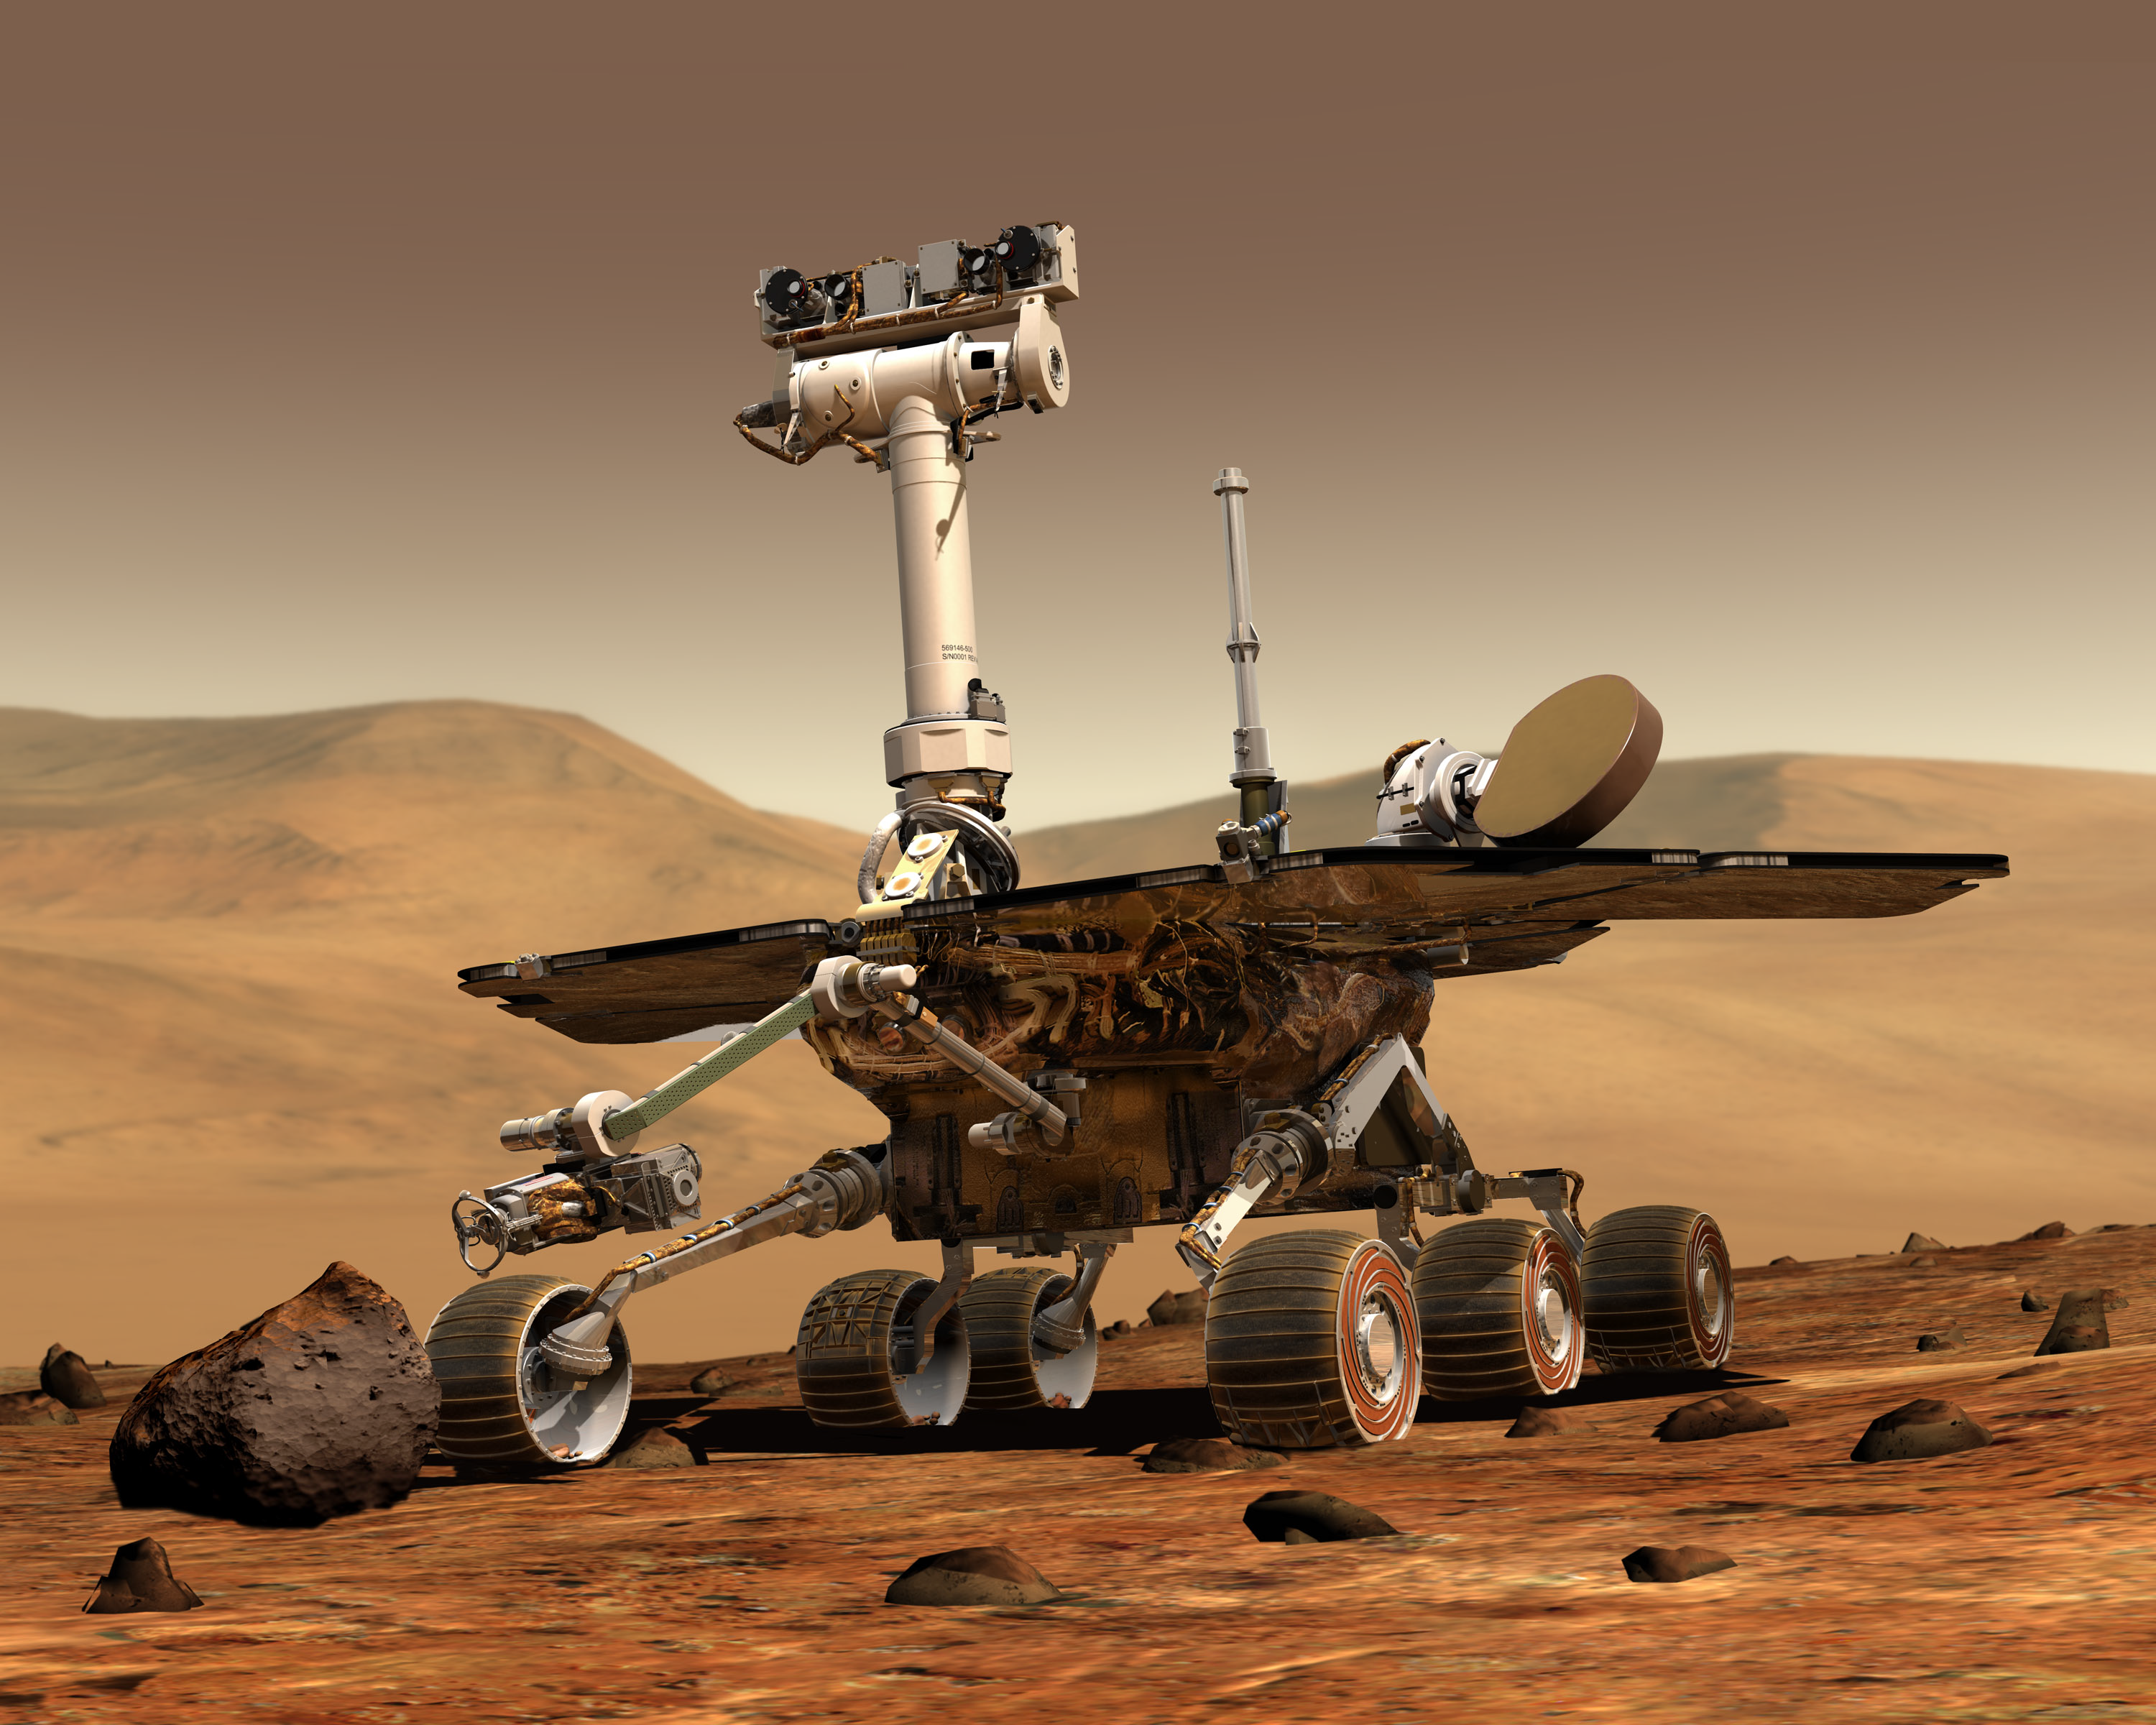
\includegraphics[width=.9\linewidth]{images/fig_01}
\end{center}
\end{minipage}
\end{exemple}

Une particule est stockée sous la forme d'un tuple de la forme \texttt{particule = (x,y,vx,vy)}.
Les particules sont stockées sous forme de listes. Un ensemble de particules est représenté par un triplet \texttt{(largeur, hauteur, listeParticules)} tel que \texttt{largeur x hauteur} sont les dimensions du rectangle et \texttt{listeParticules} est la liste des particules considérées. On considère que ces particules ont un rayon fixe et identique pour chacune d'entre elles. Le rayon est stocké dans une variable globale\footnote{Une variable globale est accessible en lecture n'importe où dans le code, même
à l'intérieur des fonctions.} nommée \texttt{rayon}.

\begin{exemple} Pour la figure ci-dessus, \texttt{listeParticules} est de la forme :
\texttt{(6, 4, [(2.2, 1.6, 0.1, 0.6), (3.25, 2.45, 0.45, 0.05), (0.2, 2.7, -0.5, -0.3),
(5.7, 3.7, 0.5, 0.6)])}.
\end{exemple}

\subsection*{Listes non triées}

Dans un premier temps, il n'y a aucune contrainte sur l'ordre des particules dans la liste. 
\subparagraph{}
\textit{Écrire une fonction \texttt{detecterCollisionEntreParticules(p1,p2)} qui prend en paramètre deux particules et renvoie \texttt{True} si les particules sont en collision et \texttt{False} sinon.}
\ifprof
\begin{corrige}
\begin{python}
def detecterCollisionEntreParticules(p1, p2): 
    x1, y1, vx1, vy1 = p1
    x2, y2, vx2, vy2 = p2
    return (x2-x1)**2+(y2-y1)**2 <= (2*rayon)**2
\end{python}
\end{corrige}
\else
\fi


\subparagraph{}
\textit{Écrire une fonction \texttt{maj(particules)} qui prend en paramètre un ensemble de particules (un triplet comme indiqué plus haut) à l'instant $t$ et renvoie un ensemble contenant des particules à l'instant $t+1$, sans s'occuper des collisions éventuelles.}
\ifprof
\begin{corrige}
\begin{python}
def deplacerParticule(particule, largeur, hauteur): # rappel de la fonction
    x, y, vx, vy = particule
    if x+vx<=0 or x+vx>=largeur: vx *= -1
    if y+vy<=0 or y+vy>=hauteur: vy *= -1
    return (x+vx, y+vy, vx, vy)
\end{python}
\end{corrige}
\else
\fi

\subparagraph{}
\textit{À l'aide de la fonction précédente, écrire une fonction \texttt{majOuCollision(particules)} qui prend en paramètre un ensemble de particules à l'instant $t$ et renvoie un ensemble contenant les particules à l'instant $t+1$, s'il n'y a pas eu de collision à l'instant $t+1$. S'il y a eu une collision la fonction renvoie \texttt{None}.}
\ifprof
\begin{corrige}
\begin{python}
def majOuCollision(particules):
    nParticules = maj(particules)
    largeur, hauteur, listeParticules = nParticules
    collision = False    
    for i in range(len(listeParticules)-1):
        for j in range(i+1, len(listeParticules)):
            if detecterCollisionEntreParticules(listeParticules[i], listeParticules[j]):
                collision = True
    if collision:
        return None
    else:
        return nParticules 
\end{python}
\end{corrige}
\else
\fi


\subparagraph{}
\textit{Écrire une fonction \texttt{attendreCollision(particules, tMax)} qui prend un ensemble de particules et un temps \texttt{tMax} en paramètres et renvoie le temps où a eu lieu la première collision entre
deux particules. S'il n'y a pas de collision avant le temps \texttt{tMax}, la fonction renvoie \texttt{None}. Quelle
est sa complexité, en fonction du nombre $n$ de particules et de \texttt{tMax} ? La réponse devra être
justifiée.}
\ifprof
\begin{corrige}
\begin{python}
def attendreCollision(particules, tMax):
    # O(n * n * tMax)
    t = 0
    while t < tMax and particules != None:
        t += 1
        particules = majOuCollision(particules)
    if t == tMax:
        return None
    else:
        return t
\end{python}
\end{corrige}
\else
\fi


\subsection*{Listes triées}

Afin d'essayer d'améliorer l'efficacité de la détection des collisions, on propose de trier la liste des
particules selon leurs abscisses. L'idée est qu'une particule \texttt{p} ne peut entrer en collision qu'avec
des particules suffisamment proches d'elle et il ne sera donc pas nécessaire de parcourir toute
la liste pour trouver les particules susceptibles d'entrer en collision avec \texttt{p}.

On rappelle que les normes des vitesses de toutes les particules sont majorées par $v_{\text{max}}$. On
supposera que l'on dispose d'une variable globale \texttt{vMax} qui contient cette valeur.

\subparagraph{}
\textit{Pour que deux particules \textbf{a} et \textbf{b} aient une chance d'entrer en collision à un instant $t+1$ donné,
à quelle distance, au maximum, devaient-elles se trouver à l'instant $t$ ? On exprimera le résultat
en fonction du \texttt{rayon} des particules et de leur vitesse maximale \texttt{vMax}.}
\ifprof
\begin{corrige}
\begin{python}

\end{python}
\end{corrige}
\else
\fi


\subparagraph{}
\textit{Écrire la fonction \texttt{majOuCollisionX(particules)}. Elle prend en paramètre un ensemble de
particules dont la liste des particules est triée par abscisses croissantes. Elle renvoie un ensemble
contenant les particules à l'instant $t+1$, sauf si une collision survient entre deux particules, auquel
cas la fonction renvoie \texttt{None}. Cette fonction devra exploiter le fait que la liste des particules est
triée pour limiter le nombre d'appels à la fonction \texttt{detecterCollisionEntreParticules}.}
\ifprof
\begin{corrige}
\begin{python}
def majOuCollisionX(particules):
    nParticules = maj(particules)
    largeur, hauteur, listeParticules = particules
    largeur, hauteur, nlisteParticules = nParticules
    collision = False
    for i in range(len(listeParticules)-1):
        j = i + 1
        while (listeParticules[j][0]-listeParticules[i][0]<=2*(vMax + rayon)) 
         and (j<len(listeParticules)-1) and not collision:   
            if detecterCollisionEntreParticules(nlisteParticules[i], nlisteParticules[j]):
                collision = True
            j += 1
    if collision:
        return None
    else:
        return nParticules 
\end{python}
\end{corrige}
\else
\fi



\end{document}
